\section{HI in anderen Galaxien}
\begin{frame}[plain,t]{THINGS – extragalaktische \SI{21}{\centi\meter}-Linien}

  The H\textsc{I} Nearby Galaxy Survey – Very Large Array: 

  \begin{columns}[c, onlytextwidth]
    \begin{column}{0.4\textwidth}
      \begin{description}[Teleskope]
        \item[Ort] New Mexico, USA
        \item[Teleskope] 27 Stück \\
          \SI{25}{\meter} Durchmesser
      \end{description}
    \end{column}
    \begin{column}{0.55\textwidth}
      \begin{description}[Messdauer]
        \item[Auflösung] \SI{7}{\arcsecond} bzw. \SI{5}{\kilo\meter\per\second}
        \item[Messung] 34 Objekte zwischen  \num{3} und \SI{15}{\mega pc}
        \item[Messdauer] $> \SI{500}{\hour}$
      \end{description}
    \end{column}
  \end{columns}
  
  
  \begin{tikzpicture}[remember picture, overlay, shift=(current page.south west)]
    \node[anchor=south] at (0.5\paperwidth, -0.4) {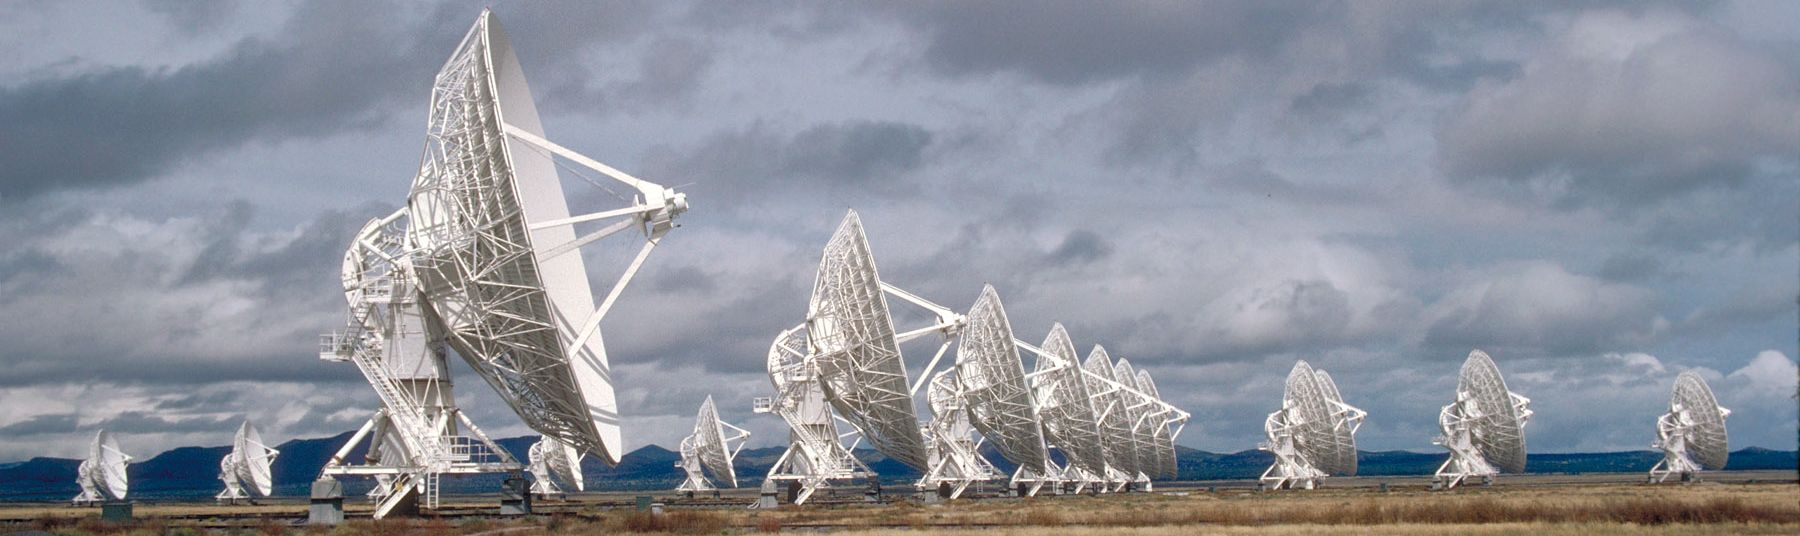
\includegraphics[width=\paperwidth]{images/vla_crop.jpg}};
  \end{tikzpicture}
\end{frame}

\fullscreenimage[\cite{things_galaxies}]{./images/things_galaxies.jpg}
\fullscreenimage[\cite{things_all}]{./images/things.png}
